%-------------------3.1
Code listing using \textit{minted} in \mybox[red]{beamer}
\begin{table}[h!]
\begin{tabular}{c | c}
\begin{minipage}[m]{0.4\textwidth}
\enum{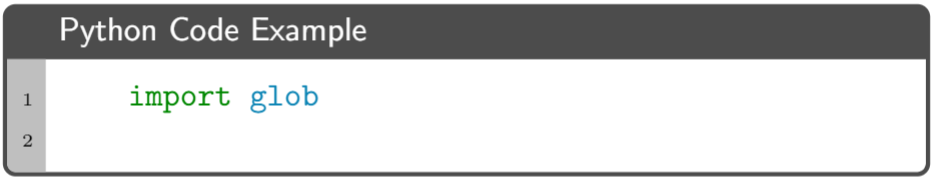
\includegraphics[width=1\linewidth]{3.1.png}}{3.1}
\end{minipage}
&
\begin{minipage}[m]{0.55\textwidth}
\begin{lstlisting}[numberstyle=\zebra{pink!15}{green!15},numbers=left,basicstyle=\footnotesize]{tex}
\documentclass{beamer}
\usepackage{amsmath}
\usepackage{tcolorbox}
\tcbuselibrary{minted,skins,breakable}
\newtcblisting{pythoncode}[2][]{
  listing engine=minted, breakable,  colback=bg,
  colframe=black!70,  listing only,
  minted style=colorful,  minted language=python,
  minted options={numbersep=3mm,texcl=true,#1},
  left=5mm,enhanced,
  overlay={\begin{tcbclipinterior}\fill[black!25] (frame.south west)
rectangle ([xshift=5mm]frame.north west);\end{tcbclipinterior}},
#2,}
\begin{document}
\begin{frame}[fragile]
    \frametitle{Premature Optimization}
    \begin{pythoncode}[linenos=true,]{title=Python Code Example}
    import glob
    \end{pythoncode}
\end{frame}
\end{document}
\end{lstlisting}
\end{minipage}
\end{tabular}
\end{table}
%-------------------3.2
\begin{table}[h!]
\begin{tabular}{c | c}
\begin{minipage}[m]{0.4\textwidth}
 \begin{lstlisting}[numberstyle=\zebra{green!25}{yellow!25},numbers=left,basicstyle=\footnotesize]
/**
* Prints Hello World.
**/
#include <stdio.h>

int main(void) {
   printf("Hello World!");
   return 0;
}
\end{lstlisting} 
\end{minipage}
&
\begin{minipage}[m]{0.55\textwidth}
\begin{footnotesize}
\begin{verbatim}
\documentclass{article}

\usepackage[T1]{fontenc}
\usepackage{beramono}
\usepackage{listings}
\usepackage{xcolor}

\newcommand\realnumberstyle[1]{}

\makeatletter
\newcommand{\zebra}[3]{%
    {\realnumberstyle{#3}}%
    \begingroup
    \lst@basicstyle
    \ifodd\value{lstnumber}%
        \color{#1}%
    \else
        \color{#2}%
    \fi
        \rlap{\hspace*{\lst@numbersep}%
        \color@block{\linewidth}{\ht\strutbox}{\dp\strutbox}%
        }%
    \endgroup
}
\makeatother
\begin{document}

\begin{lstlisting}[language=C,basicstyle=\ttfamily,
numberstyle=\zebra{green!35}{yellow!35},numbers=left]
/**
* Prints Hello World.
**/
#include <stdio.h>

int main(void) {
   printf("Hello World!");
   return 0;
}
\end{lstlisting}

\end{document}
\end{verbatim}
\end{footnotesize}
\end{minipage}
\end{tabular}
\end{table}